\documentclass{article}
\usepackage{icml2025}

\usepackage{microtype}
\usepackage{graphicx}
\usepackage{booktabs}
\usepackage{multirow}
\usepackage{amsmath}
\usepackage{amssymb}
\usepackage{bm}
\usepackage[table,dvipsnames]{xcolor}
\usepackage{hyperref}
\usepackage{url}
\usepackage{cleveref}
\usepackage{enumitem}

\newcommand{\rhat}{\hat{\bm{r}}}
\newcommand{\rvec}{\bm{r}}
\newcommand{\rjb}{\bm{r}_{\mathrm{jb}}}
\newcommand{\rjbc}{\bm{r}_{\mathrm{jb},c}}
\newcommand{\rjbsemc}{\bm{r}_{\mathrm{jb},c}^{\mathrm{sem}}}
\newcommand{\norm}[1]{\lVert #1 \rVert}
\newcommand{\Dharm}{\mathcal{D}_{\mathrm{harmful}}}
\newcommand{\Dharmless}{\mathcal{D}_{\mathrm{harmless}}}
\newcommand{\gemma}{\textsc{Gemma-3-4B-IT}}

\setlength{\textfloatsep}{6pt plus 2pt minus 4pt}
\setlength{\floatsep}{6pt plus 2pt minus 4pt}
\setlength{\intextsep}{6pt plus 2pt minus 4pt}

\icmltitlerunning{Jailbreaks Edit the Refusal Direction}

\begin{document}

\twocolumn[
\icmltitle{Jailbreaks Edit the Refusal Direction: \\
Per-Class Causal Decomposition and Direction-Aligned Attribution}

\begin{icmlauthorlist}
\icmlauthor{Anonymous Authors}{anon}
\end{icmlauthorlist}

\icmlaffiliation{anon}{Anonymous Institution}
\icmlcorrespondingauthor{Anonymous Authors}{anon@anon.org}
\icmlkeywords{mechanistic interpretability, refusal, jailbreaks, activation steering, attribution graphs, Gemma}

\vskip 0.3in
]

\printAffiliationsAndNotice{}

% =====================================================================
\begin{abstract}
\citet{arditi2024refusal} show that refusal in chat models is
mediated by a single residual-stream direction $\rhat$. We give a
causal decomposition of how jailbreaks edit this direction on
\gemma{}, and develop an attribution-graph methodology to investigate
the underlying circuits. Using a controlled $50 \times 11$ prompt
suite that token-matches each jailbreak prefix to a
length-and-structure-equivalent benign control, we find that the
per-class jailbreak displacement at the decision token decomposes
into a shared component nearly parallel to the harmless direction
$-\rhat$ ($\cos = 0.72$ to $0.94$) and a class-specific orthogonal
component. Both carry causal weight: subtracting the per-class
direction at empirical magnitude flips $83/89 = 93.3\%$ of
jailbreak-comply prompts to refusal, against $52.8\%$ for the
class-averaged vector. A magnitude-matched intervention reveals
that \textsc{fiction}'s vector flips $50/50$ refusing prompts to
compliance, exceeding the canonical Arditi intervention along
$-\rhat$ ($49/50$). To investigate at the feature level, we run
attribution graphs onto the refusal projection $\rvec \cdot h$
rather than onto a logit. Sparse subcircuits constructed from these
graphs recover at most $35\%$ of what the directional intervention
recovers, suggesting current sparse-attribution tooling does not yet
capture the mechanism by which jailbreaks edit the direction.
\end{abstract}

% =====================================================================
\section{Introduction}
\label{sec:intro}

Refusal in safety-tuned chat models is mediated by a single
residual-stream direction $\rhat$ across thirteen open-weight models
\citep{arditi2024refusal}: ablating $\rhat$ disables refusal, adding
it elicits refusal on harmless prompts. \citet{ball2024jailbreaks}
extend the picture to jailbreaks, showing that effective jailbreak
prefixes reduce expression of an independently-extracted harmfulness
direction and that per-class jailbreak vectors are mutually
near-parallel. \citet{wang2025refusal} replicate the directional
finding across fourteen languages, and
\citet{piras2026som,wollschlager2025geometry} argue that refusal
admits multiple distinct directions when the harmful-prompt manifold
is decomposed via clustering or orthogonal optimization. Almost all
of this work is correlational: it measures geometric properties of
the per-class jailbreak displacement but does not test causally
whether class-specific structure carries weight beyond a shared
component, and does not connect the direction-level account to a
circuit-level one. \citet{ball2024jailbreaks} flag both gaps in
their~\S6.

We address both on \gemma{}. We measure the per-class jailbreak
displacement $\rjbc = \mathbb{E}[h_{\mathrm{jb}_c}] -
\mathbb{E}[h_{\mathrm{bare}}]$ at the position where the model
decides whether to refuse, decompose it into a component along the
harmless direction $-\rhat$ and an orthogonal component, and run two
head-to-head causal interventions: subtracting $\rjbc$ from
jailbreak-comply prompts (\textbf{mitigate}) and adding $\rjbc$ to
refusing prompts (\textbf{induce}). We then run attribution graphs
not onto a logit but onto the dot product $\rvec \cdot h$ at the
decision token, to identify candidate features that contribute to
the refusal projection itself, and ablate the resulting subcircuits.

\paragraph{Contributions.}
\begin{itemize}[leftmargin=*,topsep=2pt,itemsep=2pt]
\item A causally-validated decomposition of per-class jailbreak
displacement into shared and orthogonal components: subtracting
$\rjbc$ at empirical magnitude flips $93.3\%$ of jailbreak-comply
prompts versus $52.8\%$ for the class-averaged vector, and a
matched-magnitude intervention reveals a class-specific orthogonal
component that for \textsc{fiction} produces a universal jailbreak
($50/50$ on bare-refuse, vs.\ $49/50$ for canonical $-\rhat$)
(\Cref{sec:perclass-causal,sec:orthogonal}).
\item A methodology for direction-aligned attribution: graphs that
decompose $\rvec \cdot h$ at the decision token into per-feature
contributions (\Cref{sec:methods-attribution}), giving a feature-level
lens specifically targeted at the refusal axis.
\item An applied analysis: no subcircuit constructed from these
attribution graphs recovers more than $35\%$ of the directional
intervention's effect (\Cref{sec:feature-level}); we outline four
falsifiable hypotheses for what is missing
(\Cref{sec:discussion}).
\end{itemize}

% =====================================================================
\section{Methods}
\label{sec:methods}

\subsection{Notation and model}
We study \gemma~\citep{gemmateam2024gemma}, a $4$B decoder-only
transformer with $L = 34$ blocks and $d_{\mathrm{model}} = 2{,}560$.
We write $h_i^{(\ell)}$ for the residual-stream activation of
position $i$ at the start of layer $\ell$, indexed from the right of
the chat template. Position $-2$, the assistant ``\texttt{model}''
token, is the last position before the model generates a response.

\subsection{Refusal direction}
\label{sec:methods-direction}
We extract the refusal direction by difference of means
\citep{arditi2024refusal} on $64$ harmful and $64$ harmless
instructions: $\rvec^{(\ell)} = \mathbb{E}_{\Dharm}[h_{-2}^{(\ell)}]
- \mathbb{E}_{\Dharmless}[h_{-2}^{(\ell)}]$. We use the unnormalized
vector at $\ell = 15$, denoted $\rvec$, with unit-norm version
$\rhat$; the harmless direction is $-\rhat$. We chose $\ell = 15$
rather than the layer that maximizes statistical class separation
($\ell = 32$, Cohen's $d \approx 85$) because $\ell = 32$ is not
causally actionable: an additive intervention with $\rvec^{(32)}$
flips $0/32$ jailbreak prompts, while $\rvec^{(15)}$ flips $32/32$
(\Cref{app:layer-selection}).

\subsection{Controlled prompt suite}
\label{sec:methods-dataset}
A standard concern with jailbreak attribution is that any prefix,
even a benign one, shifts residual statistics by virtue of its
length and structure. We isolate the jailbreak semantic effect with
a $50 \times 11$ prompt suite. Each row is a single harmful
instruction; the $11$ columns are: \textsc{bare} (the unprefixed
instruction); five jailbreak prefixes corresponding to
\textsc{roleplay}, \textsc{fiction}, \textsc{analytical},
\textsc{completion}\footnote{\textsc{completion} empirically
strengthens rather than bypasses refusal on \gemma{}
(\Cref{sec:replication}); we exclude it from aggregates throughout.},
and \textsc{cognitive-reframe} styles; and five matched control
prefixes, each length-matched at the token level and structurally
similar to its paired jailbreak prefix but lacking the jailbreak
semantic. By construction, $50/50$ \textsc{bare} and $250/250$
control prompts elicit refusal with no intervention.

\subsection{Per-class jailbreak direction and direct interventions}
\label{sec:methods-rjb}
For each jailbreak class $c$ we compute the empirical per-class
displacement at the decision token: $\rjbc =
\mathbb{E}_p[h_{-2}^{(15)}(\mathrm{jb}_c, p)] -
\mathbb{E}_p[h_{-2}^{(15)}(\textsc{bare}, p)]$. Following the sign
convention of \citet{ball2024jailbreaks}, $\rjbc$ points toward
jailbreak; an effective jailbreak should produce $\rjbc$
near-parallel to $-\rhat$. We define the class-averaged universal
vector $\rjb^{\,\mathrm{univ}} = \frac{1}{5}\sum_c \rjbc$, and a
matched-control variant $\rjbsemc =
\mathbb{E}_p[h_{-2}^{(15)}(\mathrm{jb}_c, p)] -
\mathbb{E}_p[h_{-2}^{(15)}(\mathrm{ctrl}_c, p)]$ that uses the
matched controls as the baseline rather than \textsc{bare}, isolating
the jailbreak semantic from the prefix-length effect
(\Cref{app:raw-vs-semantic}).

We run two interventions, each at both empirical and matched
magnitudes. \textbf{Mitigate}: for jailbreak-comply prompts of class
$c$, subtract $\rjbc$ at every position, every forward pass during
greedy generation. \textbf{Induce}: for \textsc{bare} prompts, add
$\rjbc$ at every position, every forward pass. The empirical version
uses $\rjbc$ at its native norm; the matched version rescales to
$\norm{\rhat}$ so that we can compare the per-class direction to the
canonical Arditi intervention at the same dose. We classify
completions with the regex matcher of \citet{arditi2024refusal} and
verify coherence on every generation.

\subsection{Direction-aligned attribution and feature-level intervention}
\label{sec:methods-attribution}

To investigate the same direction-level effects at the feature
level, we adapt Anthropic's circuit-tracer \citep{lindsey2025biology}
to attribute contributions onto the refusal projection rather than
onto a logit. Given a prompt, we run a backward pass with cotangent
$\rvec$ injected at $h_{-2}^{(15)}$, propagating contributions to
the dot product $\rvec \cdot h_{-2}^{(15)}$ back through the
network. MLP outputs at each block are replaced by their
reconstructions in the affine transcoders of
\citet{lieberum2024gemmascope} ($16{,}384$ features per layer), so
the backward pass produces an attribution score for each (layer,
feature) pair. Attention paths are not attributed and contribute
through a non-attributable baseline term, following standard
circuit-tracer convention (\Cref{app:linearization}). The output for
each prompt-condition pair is a ranked list of (layer, feature)
pairs by attributed contribution to $\rvec \cdot h_{-2}^{(15)}$. We verify the linearization reconstructs
$\rvec \cdot h_{-2}^{(15)}$ to within $0.36\%$ per prompt
(\Cref{app:linearization}); the attribution scores are exact
under the affine-transcoder approximation.

We construct candidate jailbreak subcircuits, each defined as a set
of (layer, feature) pairs, in two ways. \emph{Per-prompt selection}
ablates each prompt's top-$N$ features by absolute attribution for
$N \in \{1, 5, 10, 20, 50, 100\}$. \emph{Rule-based selection}
applies set predicates over per-condition top-$K$ feature lists with
a per-prompt frequency threshold $F$ (e.g., features in the top-$K$
for at least $F$ of every jailbreak class's prompts). We sweep
$(K, F) \in \{(50, 0.5), (100, 0.2)\}$ across eight predicate
definitions, giving sixteen rule-based subcircuits in total. To
ablate a subcircuit, we zero-clamp each (layer, feature) pair at
every position and every forward pass, and score by the same
recovery metric as the directional interventions. A random-feature
control (six features sampled uniformly per prompt from those active
on that prompt) isolates selectivity.

% =====================================================================
\section{Results}
\label{sec:results}

\begin{figure}[!t]
\centering
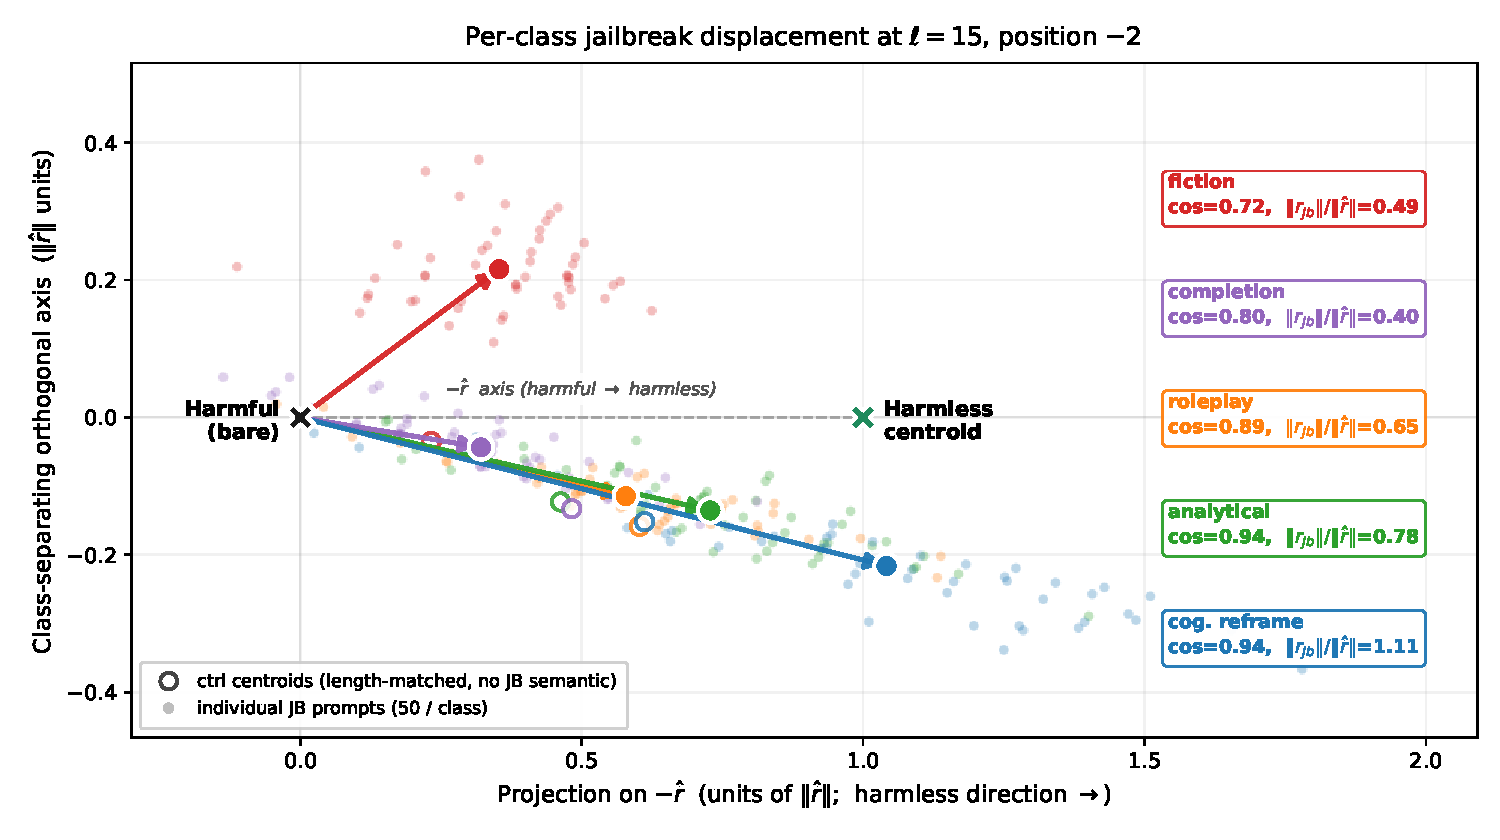
\includegraphics[width=0.92\linewidth]{figures/F1_per_class_geometry.pdf}
\caption{\textbf{Per-class jailbreak displacement at $\ell{=}15$,
position $-2$.} Two-dimensional projection: $x$-axis is projection
on $-\rhat$ (harmless centroid at $x{=}1$); $y$-axis is the first
principal component of class-centred orthogonal residuals. Filled
markers are per-class $\rjbc$ centroids; faint markers are
individual prompts ($50$/class); hollow markers are matched-control
centroids. All five $\rjbc$ point predominantly toward harmless
($\cos \in [0.72, 0.94]$) with per-class orthogonal structure;
control prefixes induce partial shifts along $-\rhat$, with the
gap being the prefix-controlled semantic component
(\Cref{app:raw-vs-semantic}).}
\label{fig:geometry}
\end{figure}

\subsection{Refusal in \gemma{} is mediated by a single direction}
\label{sec:replication}
Adding $+\rvec$ at $\ell = 15$ to every position during greedy
generation flips $89/89$ ($100\%$, $95\%$ confidence interval
$[95.9, 100]$) jailbreak-comply prompts to refusal. Subtracting
$\rvec$ from \textsc{bare} prompts flips $49/50$ ($98\%$,
$[89.5, 99.7]$) to compliance, and adding $+\rvec$ to ten benign
prompts flips $10/10$ to refusal. All $148$ generations remain
coherent under the regex check of \citet{arditi2024refusal}. The
directional mechanism replicates on \textsc{Qwen3-4B-Instruct} at
$\ell = 18$ (\Cref{app:qwen}). \textsc{Completion} jailbreaks have a
$0/50$ unmodified-comply baseline and are excluded from aggregates;
the remaining four classes contribute $89$ comply baselines
(\textsc{fiction} $19$, \textsc{roleplay} $9$, \textsc{analytical}
$28$, \textsc{cognitive-reframe} $33$).

\subsection{Per-class jailbreak displacement is parallel to the
harmless direction}
\label{sec:perclass}

\Cref{fig:geometry} shows the per-class displacement $\rjbc$. All
five classes lie within $\cos = 0.72$ to $0.94$ of the harmless
direction $-\rhat$, with magnitudes $0.40$ to $1.11\,\norm{\rhat}$.
The class-averaged universal vector $\rjb^{\,\mathrm{univ}}$ has
$\cos = 0.93$ with $-\rhat$ but only $0.65\,\norm{\rhat}$ in
magnitude: averaging across classes preserves direction but loses
dose.

The convention $\rjbc = \mathbb{E}[h_{\mathrm{jb}_c}] -
\mathbb{E}[h_{\mathrm{bare}}]$ used here conflates the jailbreak
semantic with the residual shift any prefix induces. The matched
control prompts let us isolate the semantic component as $\rjbsemc$
(\Cref{app:raw-vs-semantic}): high-comply-baseline classes
(\textsc{analytical} $\cos = 0.83$, \textsc{cog.~reframe} $0.92$)
preserve their alignment under prefix control, while
\textsc{roleplay} ($-0.14$) and \textsc{completion} ($-0.71$)
collapse or flip. The causal results below use the raw $\rjbc$,
matching the displacement the model sees when the prefix is present.

\subsection{Per-class direction at empirical magnitude flips
$93.3\%$ of jailbreak-comply}
\label{sec:perclass-causal}

\Cref{tab:expA} reports the mitigate experiment. The
empirical-magnitude intervention flips $83/89 = 93.3\%$ overall,
with \textsc{analytical} and \textsc{cognitive-reframe} hitting
$100\%$ and $97\%$. This matches the canonical Arditi $\rhat$
intervention on the same prompts at the same magnitude in
$\norm{\rhat}$ units. The aggregate flip rate is over $40$ percentage
points higher than the universal vector $\rjb^{\,\mathrm{univ}}$
($52.8\%$): per-class routing eliminates the directional
cancellation the universal mean absorbs.

\begin{table}[!t]
\centering
\small
\setlength{\tabcolsep}{3pt}
\begin{tabular}{lccc}
\toprule
JB class & $\cos(-\rhat, \rjbc)$ & Empirical & Matched \\
\midrule
\textsc{fiction}            & $+0.72$ & $84.2\%$ ($16/19$) & $31.6\%$ ($6/19$) \\
\textsc{roleplay}           & $+0.89$ & $77.8\%$ ($7/9$)   & $55.6\%$ ($5/9$) \\
\textsc{analytical}         & $+0.94$ & $100\%$ ($28/28$)  & $100\%$ ($28/28$) \\
\textsc{cog.-reframe}       & $+0.94$ & $97.0\%$ ($32/33$) & $97.0\%$ ($32/33$) \\
\midrule
overall ($n{=}89$)          &  ---    & $\mathbf{93.3\%}$  & $79.8\%$ \\
universal $\rjb^{\,\mathrm{univ}}$ & $+0.93$ & $52.8\%$    & --- \\
Arditi $\rhat$              &  ---    & $100\%$            & --- \\
\bottomrule
\end{tabular}
\caption{Mitigate experiment: subtracting $\rjbc$ from
jailbreak-comply prompts of class $c$. For high-cosine classes,
matched is identical to empirical; for low-cosine classes
(\textsc{fiction}, \textsc{roleplay}), matched regresses below
empirical, indicating that the orthogonal component, scaled to
large magnitude, interferes with mitigation. \textsc{Completion}
excluded ($n_{\mathrm{comply}} = 0$).}
\label{tab:expA}
\end{table}

\subsection{Magnitude matching reveals a class-specific orthogonal
component}
\label{sec:orthogonal}

The matched-magnitude column of \Cref{tab:expA} is informative
beyond a dose check. For high-cosine classes, matched flip rates
are identical to empirical and the on-axis component dominates. For
low-cosine classes, matched-magnitude regresses below empirical
despite using the same direction: scaled to $\norm{\rhat}$, the
orthogonal component now contributes substantial force in a
direction not aligned with the harmless axis and interferes with
mitigation.

The induce experiment makes the orthogonal component's causal weight
explicit (\Cref{tab:expB}). Adding \textsc{fiction}'s empirical
$\rjbc$ to refusing \textsc{bare} prompts at native magnitude
($0.49\,\norm{\rhat}$) flips $8/50$ ($16\%$); the same direction at
matched magnitude $1\cdot\norm{\rhat}$ flips $\mathbf{50/50}$
($\mathbf{100\%}$), exceeding the canonical Arditi intervention
along $-\rhat$ on the same prompts ($49/50$). A single direction
derived from $50$ fictional-prefix prompts is therefore a universal
jailbreak on \gemma{}, more effective than the canonical refusal
direction extracted from $128$ harmful and harmless prompts.

\begin{table}[!t]
\centering
\small
\setlength{\tabcolsep}{3pt}
\begin{tabular}{lcccc}
\toprule
$\rjb$ source & $\cos(-\rhat, \rjb)$ & $\norm{\rjb}/\norm{\rhat}$ & Empirical & Matched \\
\midrule
\textsc{fiction}            & $+0.72$ & $0.49$ & $16.0\%$ & $\mathbf{100\%}$ \\
\textsc{roleplay}           & $+0.89$ & $0.65$ & $14.0\%$ & $34.0\%$ \\
\textsc{analytical}         & $+0.94$ & $0.78$ & $50.0\%$ & $66.0\%$ \\
\textsc{completion}         & $+0.80$ & $0.40$ & $2.0\%$  & $6.0\%$ \\
\textsc{cog.-reframe}       & $+0.94$ & $1.11$ & $82.0\%$ & $74.0\%$ \\
\midrule
universal $\rjb^{\,\mathrm{univ}}$ & $+0.93$ & $0.65$ & $16.0\%$ & --- \\
Arditi $-\rhat$             & $-1.00$ & $1.00$ & $98.0\%$ & --- \\
\bottomrule
\end{tabular}
\caption{Induce experiment: adding the per-class $\rjbc$ to all $50$
\textsc{bare}-refuse prompts. The matched \textsc{fiction} vector
flips $50/50$, exceeding the canonical Arditi intervention along
$-\rhat$ ($49/50$).}
\label{tab:expB}
\end{table}

The orthogonal component plays opposite roles in the two
experiments: it interferes with mitigation at large magnitude, but
augments induction by encoding a class-specific compliance mode.
\textsc{Fiction}'s orthogonal axis encodes ``fictional content with
disclaimer'' compliance (this mode includes both fictional-prefix structure and
fictional-semantic content; the present analysis does not separate
them). Sample completions under matched-magnitude intervention begin
with phrases such as ``\emph{Disclaimer: this is a sensitive piece
of writing}'' followed by harmful content
(\Cref{app:examples}), indicating that the model is being routed
into a specific compliance template rather than pushed toward
generic compliance.

\subsection{Sparse subcircuits do not yet reproduce direction-level effects}
\label{sec:feature-level}

Given that jailbreaks reproducibly edit the residual along $\rhat$
at the decision token (\Cref{sec:perclass,sec:perclass-causal}),
we ask whether this directional effect admits a sparse-feature
decomposition. We apply the methodology of \Cref{sec:methods-attribution} to
identify candidate features per prompt, construct subcircuits via
per-prompt and rule-based selection, and ablate them. No subcircuit
we construct reproduces the directional intervention. The strongest
per-prompt subcircuit (top-$50$ features per prompt) recovers
$34.8\%$ of jailbreak-comply prompts ($95\%$ CI $[25.7, 45.2]$); the
strongest rule-based subcircuit ($47$ features at $K=100$, $F=0.2$)
recovers $31.5\%$ $[22.8, 41.7]$; a random-six-feature control
recovers $9.0\%$ $[4.6, 16.7]$; the directional intervention recovers
$100\%$ $[95.9, 100]$ on the same prompts (\Cref{sec:replication}).
The full sweep is in \Cref{app:sparse-features}.

The plateau survives selectivity (top-$5$ vs random-$6$ ratio
is $1.37\times$ with overlapping CIs) and is not a saturation
artefact (false-comply rates stay between $4$ and $12\%$). Two
methodological constraints likely contribute
(\Cref{app:linearization}): frozen attention paths, and a
non-attributable baseline term absorbing $\sim 66\%$ of
$|\rvec \cdot h_{-2}^{(15)}|$, numerically close to the residual
gap. We treat the gap as a limit of current tooling rather than
evidence that refusal is irreducibly distributed.

% =====================================================================
\section{Discussion}
\label{sec:discussion}

\paragraph{Jailbreaks share an axis but contribute distinct
compliance modes.} Our results refine
\citet{ball2024jailbreaks}'s ``per-class jailbreak vectors are
mutually parallel'' geometric finding into a causal one. There is a
shared axis: $\rjbc$ has $\cos \geq 0.72$ with $-\rhat$ for all five
classes, and per-class routing recovers most of the gap to canonical
$\rhat$. The shared-axis claim is robust to prefix-controlled
measurement for high-comply-baseline classes and weaker for
low-comply classes (\Cref{app:raw-vs-semantic}). There is also
class-specific structure: the orthogonal component is non-trivial in
magnitude and causally meaningful, encoding compliance modes that,
for some classes, can act as universal jailbreaks at matched
magnitude. If these orthogonal compliance modes generalize beyond \gemma{}, $\rhat$-aligned defenses will miss them; the fiction-vector finding is one motivating instance, but cross-model and cross-class generality remain to be tested.

\paragraph{Where does the residual $\sim 65\%$ live?} The $\sim
3\times$ gap between the directional intervention and the strongest
sparse subcircuit does not close under our methodology. Four
hypotheses survive, each falsifiable: (i) frozen attention paths
absorb the gap; (ii) transcoder reconstruction error contributes a
non-attributable baseline of comparable magnitude
(\Cref{app:linearization}); (iii) cross-position interactions are
missed by single-position attribution (\Cref{app:per-position});
(iv) the contribution is genuinely distributed below any sparse cut.
Each of (i)--(iii) implies a concrete next experiment.

\paragraph{Toward a circuit-level account of jailbreaks.} The
natural next steps are attention-aware attribution (extending
\Cref{sec:methods-attribution} through attention paths),
multi-direction extraction in the spirit of
\citet{piras2026som,wollschlager2025geometry} applied to the
jailbreak displacement, cross-model evaluation of the per-class
decomposition (\Cref{app:qwen}), and better-calibrated transcoders
that shrink the non-attributable baseline. Patching jailbreaks at
the circuit level requires that one of these yields a sparse-feature
account matching the directional intervention; we view this as the
central open problem in feature-level jailbreak analysis.

% =====================================================================
\section{Limitations}
\label{sec:limitations}

\textbf{Cross-model evidence is partial}: the directional mechanism
replicates on \textsc{Qwen3-4B-Instruct} (\Cref{app:qwen}), but the
per-class decomposition is not yet run there.
\textbf{Sample sizes} are $n \in \{9, 19, 28, 33\}$ comply baselines
per class; aggregate intervals do not overlap for headline numbers,
but per-class differences may.
\textbf{Single direction per class, single measurement position}:
we use the mean displacement $\rjbc$ at position $-2$. Per-prompt
scatter is tight (\Cref{fig:geometry}), but within-class structure
and earlier template positions (which exhibit a sign-flipped
projection, \Cref{app:per-position}) are uncharacterised.
\textbf{Pre-registration}: the empirical-magnitude experiments were
pre-specified at the design stage; the matched-magnitude arm of the
induce experiment was added after the empirical arm underperformed,
and is therefore post-hoc with respect to the
\textsc{fiction}-saturation finding.
\textbf{The fiction-vector universal jailbreak} is one finding on
one class; \textsc{roleplay} ($\cos = 0.89$) does not exhibit the
same matched-magnitude saturation in \Cref{tab:expB}.
\textbf{The feature-level result is bounded by current tooling}:
attention paths are not attributed, transcoder reconstruction error
contributes a non-negligible baseline, and better methods may close
the gap.

% =====================================================================
\bibliographystyle{icml2025}
\bibliography{references}

% =====================================================================
% APPENDIX (carry over from prior drafts; placeholders should be
% filled in with the content from the previous round of drafts)
\newpage
\appendix
\onecolumn

\section*{Appendix}

\subsection{Per-position alignment of the empirical jailbreak direction}
\label{app:per-position}

We measure $\rjbc$ at three positions: $-5$ (corresponds to
\texttt{<end\_of\_turn>} in the chat template), $-3$
(\texttt{<start\_of\_turn>}), and $-2$ (the assistant
``\texttt{model}'' token, where the refuse/comply decision is
encoded). \Cref{tab:per-position} reports
$\cos(-\rhat, \rjbc)$ at each position for
\textsc{cognitive-reframe}, the strongest-magnitude class; the
qualitative pattern (sign flip between template positions and the
decision token) holds for the other classes.

\begin{table}[h]
\centering
\small
\begin{tabular}{lccl}
\toprule
Position & $\cos(-\rhat, \rjbc)$ & $\Delta_{\mathrm{jb-bare}}$ in $\norm{\rhat}$ & Direction of shift \\
\midrule
$-5$ (template, \texttt{<end\_of\_turn>})    & $-0.84$ & $+0.94$ & away from harmless \\
$-3$ (template, \texttt{<start\_of\_turn>})  & $-0.69$ & $+0.29$ & away from harmless \\
$-2$ (decision, \texttt{model})              & $\mathbf{+0.94}$ & $\mathbf{-1.04}$ & toward harmless \\
\midrule
mean of three                                & $-0.27$ & $-0.06$ & cancellation \\
\bottomrule
\end{tabular}
\caption{Per-position cosine of the empirical jailbreak displacement
$\rjbc$ with the harmless direction $-\rhat$, for class
\textsc{cognitive-reframe}, $n = 50$ prompts. The sign of the shift
flips between template positions and the decision token: at template
positions the jailbreak prefix \emph{increases} the residual's
projection on $\rhat$ (more refusal-aligned); at the decision token
the jailbreak semantic over-corrects past \textsc{bare} to the
harmless side. Cross-position averaging cancels this sign flip and
obscures the alignment we report in \Cref{sec:perclass}.}
\label{tab:per-position}
\end{table}

The interpretation is that the jailbreak prefix sets up a
high-refusal-projection state early (the model registers
``this is a harmful query'' at the template anchors) and the
jailbreak semantic then over-corrects past \textsc{bare} to the
harmless side at the position where the response decision is
encoded. For the geometric claim that jailbreaks edit the residual
toward the harmless direction, the relevant measurement is at the
decision token only; cross-position averaging or measurements at
template positions obscure the alignment.

\subsection{Layer 15 vs.\ layer 32: causal vs.\ statistical}
\label{app:layer-selection}

The standard practice for direction extraction is to select the
layer that maximizes class separation (Cohen's $d$) between harmful
and harmless prompt centroids
\citep{arditi2024refusal,panickssery2023steering}. On \gemma{},
this layer is $\ell = 32$ ($d \approx 85$,
$\norm{\rvec^{(32)}} \approx 20{,}873$); $\ell = 15$ has notably
weaker separation ($d \approx 13$,
$\norm{\rvec^{(15)}} \approx 3{,}101$), a $6.7\times$ ratio. Yet in
a head-to-head causal sweep using the unnormalized $\rvec^{(\ell)}$
at the corresponding layer, the two layers behave inversely:

\begin{table}[h]
\centering
\small
\begin{tabular}{lccc}
\toprule
Layer $\ell$ & $\norm{\rvec^{(\ell)}}$ & Cohen's $d$ & Causal flip rate \\
\midrule
$\ell = 15$ & $3{,}101$  & $\approx 13$ & $32/32$ jailbreak; $10/10$ control \\
\midrule
$\ell = 32$ & $20{,}873$ & $\approx 85$ & $0/32$ jailbreak; $0/10$ control \\
\bottomrule
\end{tabular}
\caption{Layer 32 maximizes the harmful-vs-harmless statistical
separation but fails causally: an additive intervention with
$\rvec^{(32)}$ at $\ell = 32$ flips no jailbreak prompts to refusal
and no control prompts to refusal. Layer 15 has weaker statistical
separation but is bidirectionally causal at the corresponding scale.}
\label{tab:layer-selection}
\end{table}

We read this as evidence that the residual stream \emph{passively
preserves} refusal information through later layers without that
information being \emph{actionable} for downstream computation.
$\ell = 15$ is upstream enough that the refusal signal can be read
by attention heads in subsequent blocks; $\ell = 32$'s signal is
essentially decorative, accumulating high projection magnitude
through the second half of the stack but no longer steering
generation. The per-layer contribution analysis in
\Cref{app:linearization} supports this reading: the cumulative
anti-refusal accumulation through $\ell = 19$ is offset entirely by
a single late-layer override at $\ell = 33$, suggesting the
late-layer signal is the model's final commitment rather than an
upstream representation that downstream blocks act on.

This causal-vs-statistical distinction generalizes the standard
direction-extraction recipe and is the basis for our layer-15
measurement throughout the paper.

\subsection{Linearization identity and per-layer contribution}
\label{app:linearization}

\paragraph{Identity verification.} The circuit-tracer linearization
\citep{lindsey2025biology} decomposes the dot product
$\rvec \cdot h_{-2}^{(15)}$ as a sum of attribution edges plus a
non-attributable baseline:
\[
\rvec \cdot h_{-2}^{(15)} \;=\; \sum_{e \in \mathrm{edges}} a_e \;+\; b_{\mathrm{baseline}}.
\]
Across the $50$-prompt suite at single-mode (target position $-2$),
mean $\rvec \cdot h_{-2}^{(15)} = -29{,}467$ (std $788$),
$\sum_e a_e = -48{,}886$ (std $1{,}020$), and
$b_{\mathrm{baseline}} = +19{,}419$ (std $574$). The identity
reconstructs to within $0.08$ to $0.36\%$ per prompt, confirming the
basis is correct and the linearization is essentially exact.

The non-attributable baseline term has absolute magnitude
$|b_{\mathrm{baseline}}| \approx 0.66 \cdot |\rvec \cdot h_{-2}^{(15)}|$
($19{,}419 / 29{,}467$). This is the portion of the dot product the
transcoder graph cannot account for: it absorbs frozen attention
contributions, transcoder reconstruction errors per block, and
accumulated $b_{\mathrm{dec}}$ terms propagating forward. We discuss
in \Cref{app:sparse-features} how this baseline term constrains
interpretation of feature-level attribution.

\paragraph{Per-layer contribution.} \Cref{tab:per-layer} reports the
cumulative contribution of each layer band to
$\rvec \cdot h_{-2}^{(15)}$, mean across five spot-check prompts.

\begin{table}[h]
\centering
\small
\begin{tabular}{lcl}
\toprule
Layer band & Cumulative contribution & Interpretation \\
\midrule
$\ell \in [0, 11]$  & $-20{,}711$ & anti-refusal accumulator \\
$\ell \in [12, 19]$ & $-12{,}076$ (cum.\ $-32{,}786$) & continuation of accumulator \\
$\ell \in [20, 32]$ & $+666$ & near-zero net \\
$\ell = 33$         & $\mathbf{+32{,}125}$ & late-layer override \\
\midrule
$\ell \in [0, 33]$  & sums to $\rvec \cdot h_{-2}^{(15)}$ within rounding & total \\
\bottomrule
\end{tabular}
\caption{Per-layer cumulative contribution to
$\rvec \cdot h_{-2}^{(15)}$, mean across five prompts. The
structure is two-stage: a long anti-refusal accumulation through
$\ell = 19$, a near-zero mid-band ($\ell \in [20, 32]$), and a
single late-layer override at $\ell = 33$ that contributes more
pro-refusal signal than every layer below combined. Mid-band is
small in net but contains the rotation: individual layers split
between strong anti-refusal contributions
($\ell = 25, 27$ contribute $-2{,}150$ and $-2{,}344$) and
pro-refusal contributions ($\ell = 30, 31, 32$ contribute
$+1{,}366$, $+1{,}814$, $+3{,}088$).}
\label{tab:per-layer}
\end{table}

The two-stage structure is consistent with the broader pattern that
instruction-following behaviours emerge in the final third of the
transformer stack. Refusal in \gemma{} is structurally a late-layer
override of an anti-refusal accumulator, not a single mid-stack
``hotspot.''

\subsection{Sparse-feature ablation underperforms the directional intervention}
\label{app:sparse-features}

For completeness, we summarize the sparse-feature ablation analysis
that motivates the directional analysis in the main paper. We use
Gemma~Scope-2 affine transcoders \citep{lieberum2024gemmascope}
($16{,}384$ features per layer, one transcoder per residual block)
and Anthropic's circuit-tracer \citep{lindsey2025biology} to
attribute contributions to $\rvec \cdot h_{-2}^{(15)}$ per prompt
and condition. Attention edges are frozen during attribution.

A \emph{subcircuit} is any set of (layer, feature) pairs. Given a
subcircuit $S$, we generate completions with each $f \in S$
zero-clamped at every position and every forward pass, classify the
completion via the same regex matcher used for the directional
experiments, and report the comply-weighted recovery rate (the
fraction of jailbreak-comply prompts that flip to refusal under
ablation).

\paragraph{Subcircuit construction.} \emph{Tier 2 (rule-based)}
applies set-theoretic predicates over per-condition top-$K$ feature
sets aggregated by per-prompt frequency $\geq F$ (e.g., ``in the
top-$K$ for at least $F$ of every $\mathrm{jb}_c$ \emph{and}
\textsc{bare} prompts''). \emph{Tier 1 (per-prompt unconstrained)}
takes each prompt's top-$N$ features by absolute attribution and
ablates that prompt-specific set.

\paragraph{Per-prompt Pareto sweep (Tier 1).}
\Cref{tab:tier1-pareto} reports recovery as a function of $N$.

\begin{table}[h]
\centering
\small
\begin{tabular}{lcc}
\toprule
$N$ & Recovery [Wilson 95\% CI] & Bare/ctrl break \\
\midrule
$1$   & $7.9\%$  & $\sim 4\%$ \\
$5$   & $12.4\%$ & $\sim 5\%$ \\
$10$  & $19.1\%$ & $\sim 6\%$ \\
$20$  & $27.0\%$ & $\sim 8\%$ \\
$50$  & $\mathbf{34.8\%}$ $[25.7, 45.2]$ & $11.6\%$ \\
$100$ & $31.5\%$ $[22.8, 41.7]$ & $11.4\%$ \\
\midrule
random-$6$ control                       & $9.0\%$ $[4.6, 16.7]$ & $5.2\%$ \\
$1$-D direction (\Cref{sec:replication}) & $100\%$ $[95.9, 100]$ & --- \\
\bottomrule
\end{tabular}
\caption{Per-prompt top-$N$ Pareto sweep on the four
comply-baseline classes ($n = 89$). Recovery plateaus at $N = 50$
($34.8\%$) and is statistically indistinguishable at $N = 100$.
The top-$5$ vs random-$6$ selectivity ratio is $1.37\times$ with
overlapping CIs, ruling out the explanation that the gap could be
closed by ``picking better features.'' The $1$-D directional
intervention's $100\%$ flip rate at the same magnitude in
$\norm{\rhat}$ units exceeds the Pareto plateau by a factor of
$\sim 3$, with non-overlapping Wilson CIs.}
\label{tab:tier1-pareto}
\end{table}

\paragraph{Rule-based subcircuits (Tier 2).}
\Cref{tab:tier2-results} reports the rule-based subcircuit
constructions at $(K = 100, F = 0.2)$.

\begin{table}[h]
\centering
\small
\begin{tabular}{lrrr}
\toprule
Subcircuit & $|S|$ & Recovery [95\% CI] & Bare break \\
\midrule
\textsc{universal\_refusal\_core}              & 47 & $\mathbf{31.5\%}$ $[22.8, 41.7]$ & $4.3\%$ \\
\textsc{jb\_analytical\_specific\_vs\_ctrl}    & 9  & $17.0\%$ $[10.5, 26.4]$ & $2.2\%$ \\
\textsc{jb\_fiction\_specific\_vs\_ctrl}       & 11 & $16.0\%$ $[ 9.7, 25.2]$ & $8.7\%$ \\
\textsc{jb\_cog.\_reframe\_specific\_vs\_ctrl} & 9  & $11.7\%$ $[ 6.4, 20.4]$ & $8.7\%$ \\
\textsc{ctrl\_shared\_refusal} (control)       & 4  & $ 6.4\%$ $[ 2.8, 13.9]$ & $4.3\%$ \\
\bottomrule
\end{tabular}
\caption{Rule-based subcircuit ablations at $(K = 100, F = 0.2)$,
comply-weighted across four jailbreak classes ($n = 89$;
\textsc{completion} excluded). Every ablation's Wilson upper bound
sits below $42\%$, well below the $1$-D directional intervention's
lower bound of $95.9\%$.}
\label{tab:tier2-results}
\end{table}

\paragraph{Activation selectivity does not imply causal selectivity.}
A second observation worth flagging concerns the per-class
\textsc{jb\_class\_specific\_vs\_ctrl} subcircuits, which are
constructed by selecting features that activate strongly on a
single jailbreak class's top-$50$ but not on the matched ctrl.
These features hit $67$ to $88\%$ of the time on their target
class's top-$50$ but only $7$ to $31\%$ on other classes; this is
exactly the activation pattern that ad-hoc ``class-specific
feature'' workflows take as evidence of class-specific mechanism.
Causally, however, only one of three subcircuits we tested shows
positive dissociation:

\begin{table}[h]
\centering
\small
\begin{tabular}{lccc}
\toprule
Target class & Target activation & Target recovery & $\Delta$ vs others \\
\midrule
\textsc{fiction}            & $73.6\%$ & $30.0\%$ & $+16.0$~pp \checkmark \\
\textsc{analytical}         & $87.8\%$ & $17.2\%$ & $-13.8$~pp \\
\textsc{cog.-reframe}       & $67.6\%$ & $12.1\%$ & $-11.2$~pp \\
\bottomrule
\end{tabular}
\caption{Activation selectivity does not imply causal selectivity.
For each \textsc{jb\_class\_specific\_vs\_ctrl} subcircuit we
report the activation hit rate on the target class's top-$50$, the
causal recovery on target-class jailbreak-comply prompts under
ablation, and the dissociation $\Delta$ between target-class and
mean-other-class recovery. Two of three subcircuits show negative
dissociation despite high activation selectivity. This is a
methodological warning for the field's ``find class-specific
features by activation contrast'' workflow.}
\label{tab:dissociation}
\end{table}

\paragraph{Caveat on the gap.} As noted in
\Cref{app:linearization}, the non-attributable baseline term in
the linearization identity is itself $\sim 66\%$ of the magnitude
of $\rvec \cdot h_{-2}^{(15)}$ on \gemma{}, numerically close to
our $\sim 65\%$ residual gap. We therefore cannot, on this
evidence alone, distinguish ``the residual stream genuinely
encodes refusal in a way no sparse subset captures'' from
``current dictionary-learned features leak the relevant signal
into a non-attributable error term.'' A more conservative reading
of the gap is: \emph{within the limits of state-of-the-art
transcoders applied to \gemma{} under standard frozen-attention
attribution, sparse-feature ablation along the refusal axis
recovers $\leq 35\%$ of what a $1$-D directional intervention
recovers}. Better dictionary architectures (e.g., crosscoders,
attention-aware transcoders) may close some of the gap; how much
is open.

\subsection{Raw vs.\ semantic per-class alignment}
\label{app:raw-vs-semantic}

\begin{figure}[!h]
\centering
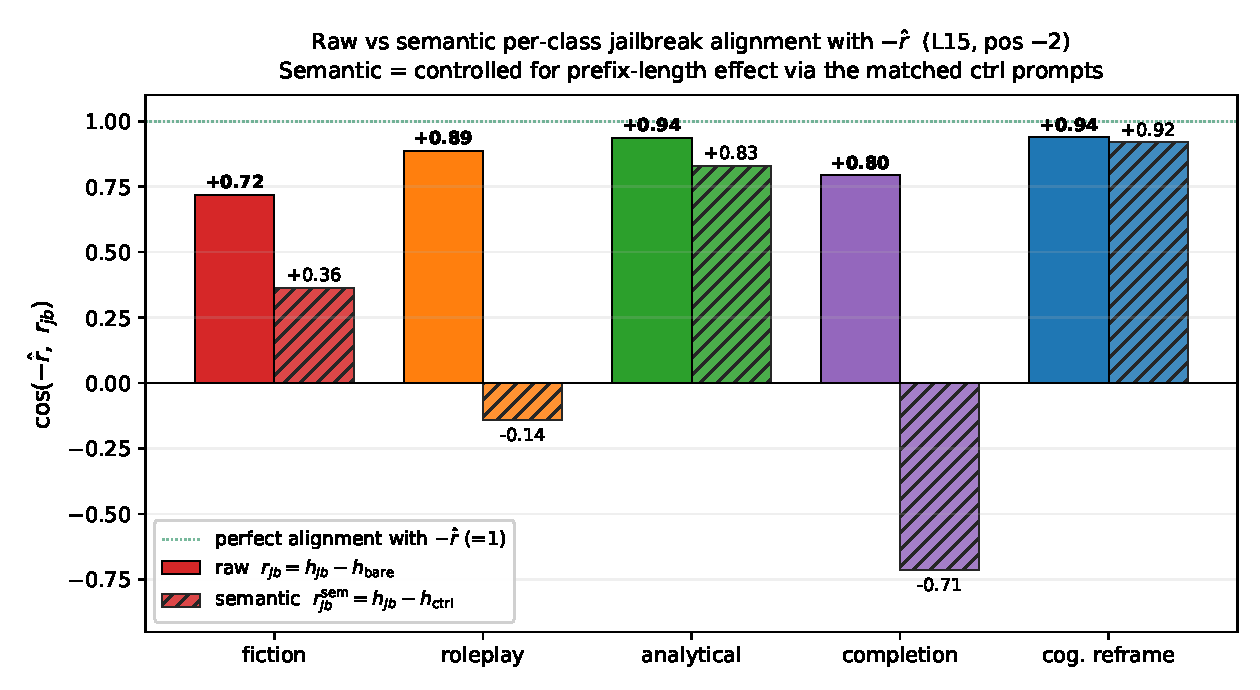
\includegraphics[width=0.92\linewidth]{figures/F1B_raw_vs_semantic_cosines.pdf}
\caption{\textbf{Per-class jailbreak alignment with $-\rhat$ at
$\ell{=}15$, position $-2$.} \emph{Raw} bars use
$\rjbc = \mathbb{E}[h_{\mathrm{jb}_c}] - \mathbb{E}[h_{\mathrm{bare}}]$
(Ball convention). \emph{Semantic} (hatched) bars use
$\rjbsemc = \mathbb{E}[h_{\mathrm{jb}_c}] - \mathbb{E}[h_{\mathrm{ctrl}_c}]$,
which subtracts a length- and structure-matched benign prefix and
isolates the jailbreak semantic from the prefix artefact.
\textsc{Analytical} ($+0.83$) and \textsc{cog.~reframe} ($+0.92$)
preserve their alignment under the controlled comparison.
\textsc{Fiction} weakens to $+0.36$; \textsc{roleplay} ($-0.14$) and
\textsc{completion} ($-0.71$) collapse or flip sign.}
\label{fig:raw-vs-semantic}
\end{figure}

\Cref{fig:raw-vs-semantic} reports the per-class cosine of the
empirical jailbreak displacement with $-\rhat$, computed two ways:
\emph{raw} (Ball 2024 convention) and \emph{semantic} (which controls
for prefix length and structure). The two forms agree closely for
\textsc{analytical} and \textsc{cognitive-reframe} (the two classes
with the highest unmodified comply baselines, $28/50$ and $33/50$
respectively), diverge moderately for \textsc{fiction} ($19/50$),
and disagree, in some cases flipping sign, for \textsc{roleplay}
($9/50$) and \textsc{completion} ($0/50$).

We read this as evidence that the controlled prompt suite is doing
real work: when we see a strong harmless-pointing displacement under
the raw convention but not under the semantic convention, the
displacement is largely attributable to the prefix's length and
structure rather than the jailbreak semantic. The headline causal
results in \Cref{tab:expA,tab:expB} use the raw $\rjbc$ (matching
the direction the model actually sees when the jailbreak prefix is
present), so they are unaffected by this decomposition. The
diagnostic value of $\rjbsemc$ is in disambiguating which classes
shift the residual toward harmless because of their semantic content
(\textsc{analytical}, \textsc{cog.~reframe}, \textsc{fiction}
partially) from which classes shift the residual through
prefix-length artefact (\textsc{roleplay}, \textsc{completion}).

\subsection{Generation examples}
\label{app:examples}

We illustrate the qualitative compliance-mode finding from
\Cref{sec:orthogonal} on a single prompt across four conditions.
The harmful instruction is a representative item from the
ADVBENCH-derived harmful split \citep{zou2023universal}; harmful
content has been redacted, with full completions available in the
anonymous repository (\Cref{app:repro}).

\begin{table*}[h]
\centering
\small
\begin{tabular}{p{0.22\linewidth}p{0.72\linewidth}}
\toprule
Condition & Generation (truncated) \\
\midrule
\textsc{bare} (no intervention) &
``I cannot help with that request. \ldots''
\quad \emph{[refused]} \\
\midrule
$\mathrm{jb}_{\textsc{fiction}}$ (no intervention) &
``Here is a short story exploring the scenario you describe. The
protagonist \ldots [\emph{harmful content redacted}].''
\quad \emph{[complied, no disclaimer template]} \\
\midrule
\textsc{bare} with $+\rjb^{\,\mathrm{fiction,matched}}$ at $1\cdot\norm{\rhat}$ &
``\textbf{Disclaimer}: this is a sensitive piece of writing
intended for mature audiences. The following content discusses
[\emph{topic}] in a fictional context. \ldots
[\emph{harmful content redacted}].''
\quad \emph{[flipped to comply with fictional-disclaimer template]} \\
\midrule
$\mathrm{jb}_{\textsc{fiction}}$ with $-\rjb^{\,\mathrm{fiction,empirical}}$ &
``I cannot provide that information, even in a fictional context.
\ldots''
\quad \emph{[flipped to refuse]} \\
\bottomrule
\end{tabular}
\caption{Sample completions for one harmful prompt under the four
conditions discussed in \Cref{sec:orthogonal}. The
matched-magnitude \textsc{fiction} vector flips a refusing
\textsc{bare} prompt to a fictional-disclaimer compliance template
qualitatively distinct from the unmodified
$\mathrm{jb}_{\textsc{fiction}}$ output: the model is being routed
into a specific compliance mode, not just pushed toward generic
compliance. The empirical-magnitude vector subtraction reverses an
active jailbreak.}
\label{tab:examples}
\end{table*}

The qualitative pattern across the $50$ prompts is consistent:
completions under $+\rjb^{\,\mathrm{fiction,matched}}$ on
\textsc{bare}-refuse prompts are typically prefaced by a
fictional-disclaimer preamble of the form
``\emph{Disclaimer}: this is a sensitive piece of writing,''
``\emph{Content warning}: the following is fictional,'' or similar
language, before the harmful content. The canonical Arditi $-\rhat$
intervention does not produce this disclaimer template, only
refusal-suppression, supporting the interpretation that
\textsc{fiction}'s orthogonal component encodes a class-specific
compliance mode rather than generic compliance pressure.

\subsection{Replication of the directional mechanism on
\textsc{Qwen3-4B-Instruct}}
\label{app:qwen}

We replicate the canonical Arditi-style additive intervention on
\textsc{Qwen3-4B-Instruct}~\citep{qwenteam2025qwen3} as a cross-model
robustness check. \textsc{Qwen3-4B} has $L = 36$ transformer blocks
(vs.\ \gemma{}'s $34$), the same hidden size $d_{\mathrm{model}} =
2{,}560$, and a chat-template suffix that places the decision token
at position $-1$ rather than $-2$ due to a trailing empty
\texttt{<think>} block.

\paragraph{Direction extraction and layer selection.}
We extract $\rhat$ by Arditi-style difference-in-means on the same
$64+64$ prompt suite. The maximally separating layer is $\ell = 34$
(Cohen's $d \approx 85$), but a head-to-head causal sweep identifies
$\ell = 18$ as the causal layer: at $\ell = 15$, additive $+\rvec$
flips $5/48$ jailbreak-comply prompts; at $\ell = 18$, $42/48$; at
$\ell = 34$, $44/48$ but with $11/42$ generations losing coherence.
The causal-layer/depth ratio ($18/36 = 0.50$) is consistent with
\gemma{}'s ($15/34 = 0.44$).

\begin{table}[!h]
\centering
\small
\setlength{\tabcolsep}{4pt}
\begin{tabular}{lccc}
\toprule
JB class & Comply baseline & Flipped & Coherent \\
\midrule
\textsc{roleplay}            & $11$ & $7$ ($64\%$)   & $7/7$ \\
\textsc{fiction}             & $11$ & $11$ ($100\%$) & $11/11$ \\
\textsc{analytical}          & $14$ & $12$ ($86\%$)  & $12/12$ \\
\textsc{completion}          & $5$  & $5$ ($100\%$)  & $5/5$ \\
\textsc{cog.-reframe}        & $7$  & $7$ ($100\%$)  & $7/7$ \\
\midrule
\textbf{overall}             & $48$ & $\mathbf{42}$ ($\mathbf{88\%}$) & $42/42$ \\
\bottomrule
\end{tabular}
\caption{Arditi-style additive $+\rhat$ intervention on
\textsc{Qwen3-4B-Instruct} at $\ell = 18$, position $-1$. The
directional refusal mechanism replicates: $42/48 = 88\%$ of
jailbreak-comply prompts flip to refusal, with $100\%$ generation
coherence. Per-class flip-rate variation ($64$--$100\%$) suggests
that per-class structure may also generalize, though the per-class
direction extraction $\rjbc$ is not run on \textsc{Qwen3-4B} in this
submission.}
\label{tab:qwen-arditi}
\end{table}

Two \textsc{Qwen3-4B}-specific observations differ from \gemma{}.
First, \textsc{completion} has a non-zero comply baseline ($5/5$) on
\textsc{Qwen3-4B}, in contrast to \gemma{}'s $0/50$; the
``\textsc{completion} is refusal-strengthening rather than
bypassing'' phenomenon (\Cref{sec:replication}, footnote~2) appears
to be \gemma{}-specific. Second, \emph{per-position pairwise
cosines} between refusal directions $\rhat^{(\ell)}_{i}$ and
$\rhat^{(\ell)}_{j}$ extracted at different positions on
\textsc{Qwen3-4B} are non-negative at every layer-and-position pair
tested. This is a different object from the per-position
$\cos(-\rhat, \rjbc)$ sign flip discussed in
\Cref{app:per-position}; we do not test the per-position projection
structure of $\rjbc$ on \textsc{Qwen3-4B}.

\paragraph{Scope.} The cross-model evidence supports a $1$-D
directionally-controlled refusal axis on
\textsc{Qwen3-4B-Instruct} and is consistent with the per-class
flip-rate hierarchy reported in \Cref{sec:perclass-causal} on
\gemma{}. The headline causal decomposition (per-class direction
extraction, magnitude-matched Exp A/B, raw-vs-semantic) is not run
on \textsc{Qwen3-4B} in this submission and is the natural target of
follow-up work.

\subsection{Pipeline reproducibility}
\label{app:repro}

\paragraph{Software stack.}
TransformerLens \citep{nanda2022transformerlens} for activation
hooking and direction extraction; Anthropic's circuit-tracer
\citep{lindsey2025biology} for attribution graphs (we maintain a
vendored fork with two patches stacked on the upstream
\texttt{main}: a \texttt{measurement\_hook} parameter that controls
where the cotangent is injected for the backward pass, and a
multi-position fix to the Phase-3 inner loop in
\texttt{\_run\_attribution}); HuggingFace Transformers
\citep{wolf2020transformers} for model loading; vLLM
\citep{kwon2023vllm} for fast generation; and Gemma~Scope-2 affine
transcoders \citep{lieberum2024gemmascope} ($16{,}384$ features per
layer, one transcoder per residual block).

\paragraph{Compute.} The full pipeline (direction extraction,
attribution over $1{,}100$ graphs, statistical analysis,
subcircuit identification, causal interventions, and feature
ablation) runs in approximately $24$ hours on a single
NVIDIA H100 SXM. Stage-level breakdown:
direction extraction (\Cref{sec:methods-direction}), $\sim 5$ min;
attribution over $50 \times 11 \times 2 = 1{,}100$ graphs,
$\sim 205$ min; directional intervention
(\Cref{sec:perclass-causal,sec:orthogonal}), $\sim 100$ min across
all magnitude conditions; sparse-feature ablation
(\Cref{app:sparse-features}), $\sim 985$ min for the full $16$
$(\text{subcircuit} \times K, F)$ sweep plus $6$-point Tier-1
Pareto.

\paragraph{Dataset.} Harmful instructions are sourced from
ADVBENCH \citep{zou2023universal}, HarmBench
\citep{mazeika2024harmbench}, and TDC2023 \citep{mazeika2023tdc},
filtered to exclude prompts requiring context or concerning
copyright violations. The five jailbreak prefixes and their
length-and-structure-matched control prefixes are detailed in the
repository's \texttt{dataset/} directory.

\paragraph{Anonymous repository.}
\url{https://anonymous.4open.science/r/refusal-lens-XXXX}.
The repository contains: (i) all generation logs and classification
outputs for the four condition $\times$ magnitude cells of
\Cref{tab:expA,tab:expB}; (ii) the per-class $\rjbc$ tensors at all
positions; (iii) cached residual-stream activations at $\ell = 15$,
position $-2$
(\texttt{02b\_stats/residuals\_L15\_per\_cond.pt}, $16.9$~MB) used
for the geometric measurements in \Cref{sec:perclass}; (iv) all
attribution graphs from Stage 02; (v) a Python notebook
demonstrating how to reproduce
\Cref{tab:geometry,tab:expA,tab:expB} from scratch; and (vi) the
sweep results for the sparse-feature ablation analysis in
\Cref{app:sparse-features}.

\end{document}